% =============================================================================
% COPYRIGHT AND DISCLAIMER
% =============================================================================
% This file is provided as a convenience template for competition participants.
% By using it, you accept full responsibility for compliance with all applicable
% copyright, licensing, and usage rules of the Association for Computing
% Machinery (ACM) and of any LaTeX packages you load (including, without
% limitation, the "acmart" document class and related ACM materials).
%
% Consult ACM's official publication, template, and copyright policies before
% using this setup for any purpose other than this competition. Do not assume
% that this template may be reused, redistributed, or submitted elsewhere
% without independently verifying ACM's current rules.
%
% Use of the "acmart" class, the "sigconf" option, or ACM-style formatting in
% this template does NOT mean that this report, this competition, its organizers,
% or any resulting PDF is sponsored, endorsed, affiliated with, or published by
% ACM. ACM trademarks and branding remain the property of ACM.
%
% Template packages live in preamble.tex.
% Citations live in main.bib. Edit this file with your paper content.
% =============================================================================

\documentclass[sigconf]{acmart}
% =============================================================================
% Template setup — participants normally do not edit this file.
% Author content belongs in main.tex; citations belong in main.bib.
% \documentclass lives in main.tex so Overleaf does not treat this file as root.
% =============================================================================

% --- Competition / non-ACM-submission friendly rights metadata -------------
\setcopyright{none}
\settopmatter{printacmref=false}
\acmConference[Kaggle Competition]{Filament Segmentation Challenge}{2026}{\href{https://www.kaggle.com/competitions/filament-segmentation-2026}{kaggle.com/competitions/filament-segmentation-2026}}
\acmBooktitle{Competition Report}
\acmDOI{}
\acmISBN{}

% --- Author guidance text --------------------------------------------------
% \guide{...} is gray italic while \guideStyletrue; omitted from the PDF if false.
% Flip the switch in main.tex after % =============================================================================
% Template setup — participants normally do not edit this file.
% Author content belongs in main.tex; citations belong in main.bib.
% \documentclass lives in main.tex so Overleaf does not treat this file as root.
% =============================================================================

% --- Competition / non-ACM-submission friendly rights metadata -------------
\setcopyright{none}
\settopmatter{printacmref=false}
\acmConference[Kaggle Competition]{Filament Segmentation Challenge}{2026}{\href{https://www.kaggle.com/competitions/filament-segmentation-2026}{kaggle.com/competitions/filament-segmentation-2026}}
\acmBooktitle{Competition Report}
\acmDOI{}
\acmISBN{}

% --- Author guidance text --------------------------------------------------
% \guide{...} is gray italic while \guideStyletrue; omitted from the PDF if false.
% Flip the switch in main.tex after % =============================================================================
% Template setup — participants normally do not edit this file.
% Author content belongs in main.tex; citations belong in main.bib.
% \documentclass lives in main.tex so Overleaf does not treat this file as root.
% =============================================================================

% --- Competition / non-ACM-submission friendly rights metadata -------------
\setcopyright{none}
\settopmatter{printacmref=false}
\acmConference[Kaggle Competition]{Filament Segmentation Challenge}{2026}{\href{https://www.kaggle.com/competitions/filament-segmentation-2026}{kaggle.com/competitions/filament-segmentation-2026}}
\acmBooktitle{Competition Report}
\acmDOI{}
\acmISBN{}

% --- Author guidance text --------------------------------------------------
% \guide{...} is gray italic while \guideStyletrue; omitted from the PDF if false.
% Flip the switch in main.tex after \input{preamble}.
%
% Do not use \guide{...} for \email{...}.
\usepackage{xcolor}
\newif\ifguideStyle
\guideStyletrue
\newcommand{\guide}[1]{%
  \ifguideStyle
    {\color{gray!65}\itshape #1}%
  \fi
}

% --- Math ------------------------------------------------------------------
% Do NOT load amssymb (or amsfonts): acmart already loads newtxmath, which
% defines the same symbols (e.g. \Bbbk) and causes a conflict on Overleaf.
% amsmath is already provided by acmart; mathtools extends it.
\usepackage{mathtools}

% --- Figures ---------------------------------------------------------------
% graphicx is already loaded by acmart
\usepackage{subcaption}

% --- Tables ----------------------------------------------------------------
% booktabs is already loaded by acmart
\usepackage{tabularx}
\usepackage{multirow}

% --- Bibliography style is set in main.tex (ACM-Reference-Format) ----------
.
%
% Do not use \guide{...} for \email{...}.
\usepackage{xcolor}
\newif\ifguideStyle
\guideStyletrue
\newcommand{\guide}[1]{%
  \ifguideStyle
    {\color{gray!65}\itshape #1}%
  \fi
}

% --- Math ------------------------------------------------------------------
% Do NOT load amssymb (or amsfonts): acmart already loads newtxmath, which
% defines the same symbols (e.g. \Bbbk) and causes a conflict on Overleaf.
% amsmath is already provided by acmart; mathtools extends it.
\usepackage{mathtools}

% --- Figures ---------------------------------------------------------------
% graphicx is already loaded by acmart
\usepackage{subcaption}

% --- Tables ----------------------------------------------------------------
% booktabs is already loaded by acmart
\usepackage{tabularx}
\usepackage{multirow}

% --- Bibliography style is set in main.tex (ACM-Reference-Format) ----------
.
%
% Do not use \guide{...} for \email{...}.
\usepackage{xcolor}
\newif\ifguideStyle
\guideStyletrue
\newcommand{\guide}[1]{%
  \ifguideStyle
    {\color{gray!65}\itshape #1}%
  \fi
}

% --- Math ------------------------------------------------------------------
% Do NOT load amssymb (or amsfonts): acmart already loads newtxmath, which
% defines the same symbols (e.g. \Bbbk) and causes a conflict on Overleaf.
% amsmath is already provided by acmart; mathtools extends it.
\usepackage{mathtools}

% --- Figures ---------------------------------------------------------------
% graphicx is already loaded by acmart
\usepackage{subcaption}

% --- Tables ----------------------------------------------------------------
% booktabs is already loaded by acmart
\usepackage{tabularx}
\usepackage{multirow}

% --- Bibliography style is set in main.tex (ACM-Reference-Format) ----------


% Guide styling: \guideStyletrue = show gray italic hints; \guideStylefalse = omit them
% \guideStyletrue
\guideStylefalse

\begin{document}

\title{Detect, then Segment: Box-Conditioned Per-Filament U-Net on Full-Resolution Crops}  % Replace this with your title
\subtitle{A Solution to the Solar Filament Segmentation Challenge 2026} % DO NOT CHANGE


\author{Vincent Liu}
\affiliation{%
  \city{TODO City}
  \country{TODO Country}
}
\email{TODO@example.com}   % <- Replace with your own email

\begin{abstract}
    This report describes our solution to the Solar Filament Segmentation Challenge~2026, a Kaggle competition on automatic segmentation of solar filaments in GONG H-$\alpha$ observations. We use a two-stage pipeline: a YOLO11 detector proposes one box per filament, and a U-Net with a ResNet-34 encoder segments each filament from a full-resolution crop around its box, conditioned on a box-mask input channel. On a month-grouped validation split the pipeline reaches a panoptic quality (PQ) of 0.448, against 0.403 for a single global U-Net with connected-component post-processing, and 0.39 on the public leaderboard. With ground-truth boxes the segmenter reaches PQ 0.686, so detection is the bottleneck; we show that this ceiling is largely set by the labels, as two annotators of the same image agree on only 58\% of filaments at IoU\,$>$\,0.5. Code, weights and a reproducibility notebook: \url{https://github.com/blueclowd/solar_filaments_segmentation}.
\end{abstract}

\maketitle


% ==================================== %
%              INTRODUCTION            %
% ==================================== %
\section{Introduction}
    This report goes over the details of our submitted solution to the Solar Filament Segmentation Challenge~2026 \cite{filament-segmentation-2026}. The challenge, launched on July~10,~2026, is organized by the Earth-Space AI Research (ESAIR) Lab\footnote{\href{https://www.esairlab.com/home}{www.esairlab.com/}}. This challenge utilizes the MAGFiLO dataset for evaluation of the segmentation algorithms \cite{ahmadzadeh2024dataset}.

    The task is class-agnostic instance segmentation: every filament is returned as a separate mask and scored by PQ \cite{kirillov2019panoptic} with one-to-one matching at IoU\,$>$\,0.5 (PQ\,=\,SQ\,$\times$\,RQ, segmentation times recognition quality). Filaments are long, thin and sparse: at 1024-pixel resolution the median bounding box has a short side of 26\,px, 21\% of boxes are under 16\,px, and a filament fills a median 20\% of its own box. A single semantic mask followed by connected components therefore struggles with both the thin shapes and the instance boundaries (where one filament ends and the next begins). Our solution separates the two problems: a detector decides \emph{where} each filament is, and a second network decides its \emph{shape} at full resolution.

% ==================================== %
%              METHODOLOGY             %
% ==================================== %
\section{Methodology}\label{sec:methodology}

\begin{figure*}[t]
    \centering
    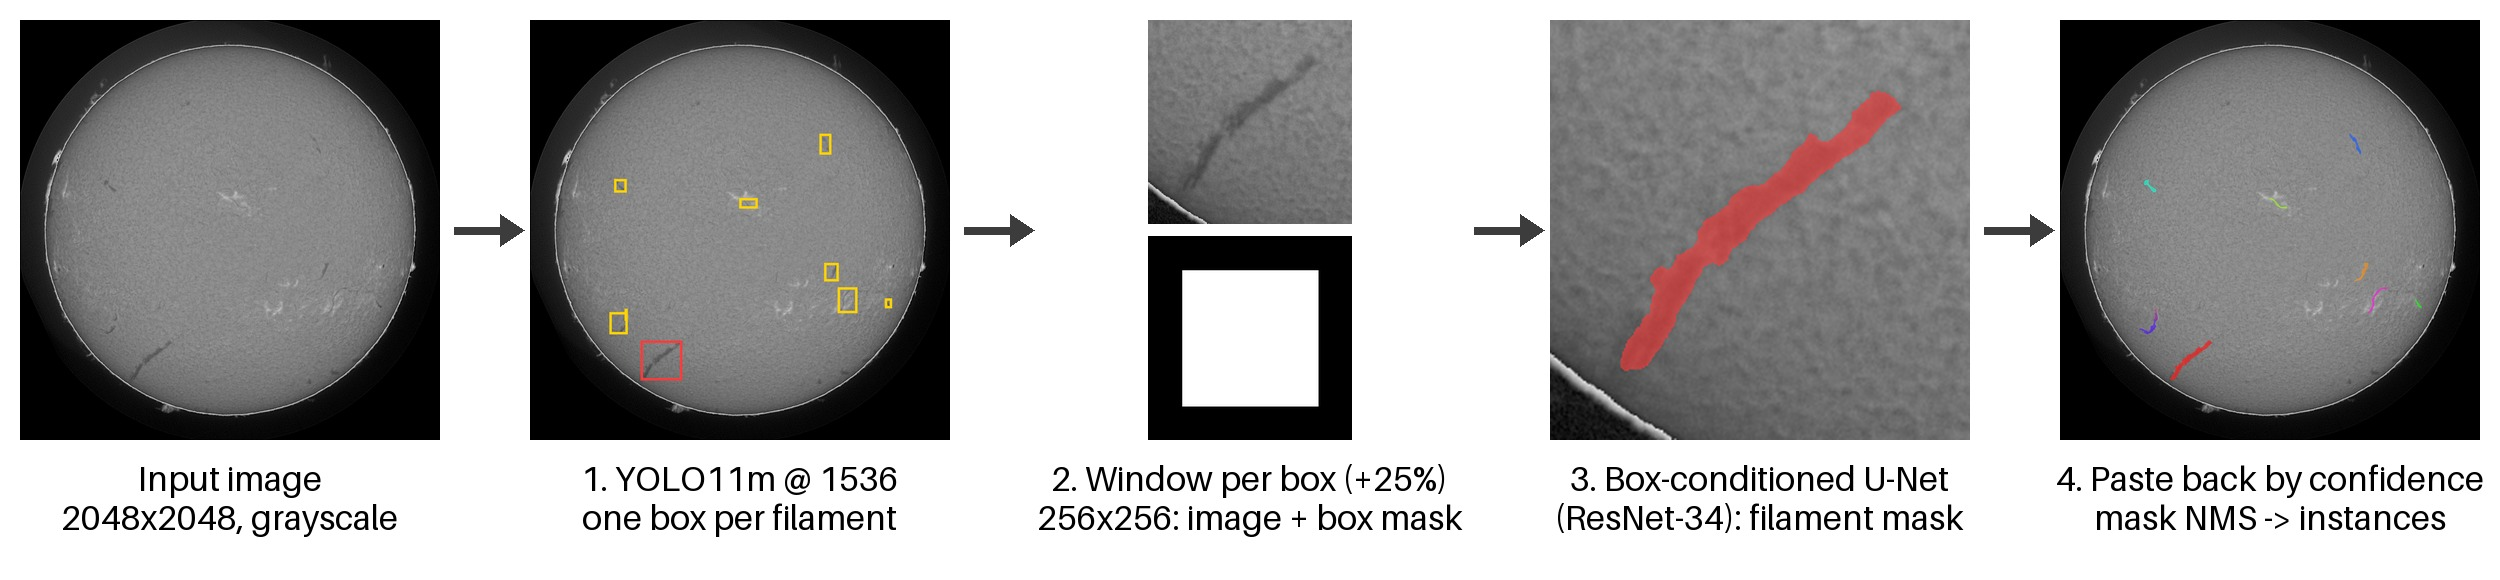
\includegraphics[width=\textwidth]{figures/pipeline.jpg}
    \caption{End-to-end pipeline, illustrated on a test image with the final predictions. (1) YOLO11m proposes one box per filament. (2) For each box, a window (box enlarged by 25\% per side) is cut from the 2048$\times$2048 image and resized to 256$\times$256; a binary box mask is the second input channel. (3) A U-Net segments the filament inside the box. (4) Masks are pasted back from the most to the least confident box, with mask-level NMS removing duplicates.}
    \label{fig:pipeline}
\end{figure*}

\subsection{Data, annotators and splits}
    The training set has 707 grayscale images of 2048$\times$2048\,px; they are read as single-channel images. The chirality classes are not scored and are merged into one \emph{filament} class; only the segmentation masks are used for training (no spines, classes or other metadata). 296 images were annotated independently by two or more people, giving 1{,}154 annotation sets. We group annotation sets by file name, so an image never appears in both training and validation. Because filaments persist for days and neighbouring images are near-duplicates, the validation split is grouped by calendar month (15\% of images, fixed seed): 594 training images (962 annotation sets, 6{,}942 filaments) and 113 validation images (192 sets, 1{,}257 filaments). For training, each annotation set is a separate sample. On validation, each annotation set is scored as its own ground truth and PQ is pooled over all of them. After model selection, both stages are retrained on all 707 images with identical settings.

\subsection{Stage 1: filament detection}
    An Ultralytics YOLO11m detector \cite{jocher2024yolo11} with a single class is trained at 1536\,px input for 150 epochs, with one label file per annotation set. Augmentation uses horizontal and vertical flips (valid once chirality classes are merged), brightness jitter, scale jitter of 0.25, mosaic, and no hue or saturation jitter (grayscale data) or rotation. Training on 1{,}154 annotation sets takes 3.1\,h on one NVIDIA A10.

\subsection{Stage 2: box-conditioned per-filament segmentation}
    For each box, a window is cut from the \emph{full-resolution} image: the box enlarged by 25\% on each side, at least 48\,px, with its aspect ratio limited to 2:1, then resized to 256$\times$256. The network input has two channels: the image crop and a binary mask of the box (Fig.~\ref{fig:pipeline}). The box channel tells the network \emph{which} filament to segment when several are in view; the target is that single filament's mask. The model is a U-Net \cite{ronneberger2015unet} from \texttt{segmentation\_models\_pytorch} \cite{iakubovskii2019smp} with an ImageNet-pretrained ResNet-34 encoder \cite{he2016resnet} and scSE decoder attention \cite{roy2018scse}, trained for 20 epochs with BCE plus soft Dice loss, AdamW \cite{loshchilov2019adamw} (learning rate $3\cdot10^{-4}$, cosine schedule with one warm-up epoch), batch size 32 and mixed precision. Ground-truth boxes are jittered during training (Gaussian, $\sigma$ = 10\% of the box side) so the network tolerates imperfect detections. Each training sample is one filament from one annotation set (8{,}199 samples on all data); an epoch takes 33\,s on one A10.

\subsection{Instance assembly and post-processing}
    Each crop is predicted with horizontal and vertical flip test-time augmentation and the probability map is pasted back into the 2048$\times$2048 frame. Boxes are processed from the most to the least confident. A mask whose IoU with an already accepted mask exceeds the NMS threshold is dropped as a duplicate, and pixels claimed by two filaments go to the higher probability. Masks below a minimum area are removed. The detector confidence threshold, mask threshold, mask-NMS IoU and minimum area are tuned on validation by coordinate search, reusing cached per-box probabilities so each setting only re-runs the assembly. The selected values are 0.3, 0.6, 0.3 and 200\,px. Inference takes 0.31\,s per image on one A10 (YOLO plus all crops, with flip TTA).

\subsection{Baseline: global U-Net}
    For comparison, a single U-Net (same encoder) segments all filament pixels of an image resized to 1024\,px, trained on 512$\times$512 crops for 30 epochs. Instances are obtained by thresholding (0.8, tuned), morphological closing, connected components, a minimum area, and merging components closer than 12\,px.

% ==================================== %
%              EVALUATION              %
% ==================================== %
\section{Evaluation}\label{sec:evaluation}

\subsection{Strategy}
    All model selection and tuning use the month-grouped validation split, with every annotation set scored separately (Sec.~\ref{sec:methodology}). We report pooled PQ, SQ and RQ, false positives (FP), false negatives (FN), and the number of ground-truth filaments split into several predictions or predictions merging several filaments. To separate detection from segmentation errors, we also score the segmenter with ground-truth boxes (\emph{oracle}). Public leaderboard scores are reported for submitted versions.

\subsection{Annotator agreement}
    To understand the ceiling, we matched the annotation sets of every multi-annotator image against each other with the competition rule. Of 4{,}086 drawn filaments, only 58.4\% have a match in the other set (Table~\ref{tab:agreement}, 95\% bootstrap intervals over images; Fig.~\ref{fig:agreement}). Box-level precision and recall between annotators are 0.615 and 0.609. We therefore keep one training sample per annotation set instead of fusing the annotators: a filament drawn by one of two annotators is a positive in half of the samples and background in the other half, so the detector learns a confidence near 0.5 for it, which is the calibration PQ needs when the reference comes from a single annotator.

\begin{table}[t]
    \caption{Agreement between two annotators of the same image (296 images, 4{,}086 filaments, matching at mask IoU\,$>$\,0.5). 95\% bootstrap confidence intervals over images.}
    \label{tab:agreement}
    \small
    \begin{tabularx}{\columnwidth}{Xc}
        \toprule
        Filaments & Share (95\% CI) \\
        \midrule
        Matched in the other annotation set & 58.4\% (56.1--60.8) \\
        Same filament, outlines differ (IoU\,$\le$\,0.5) & 14.0\% (12.5--15.6) \\
        Drawn as a different number of pieces & 10.1\% (8.4--11.7) \\
        Drawn by one annotator only & 17.5\% (16.0--19.2) \\
        \bottomrule
    \end{tabularx}
\end{table}

\begin{figure}[t]
    \centering
    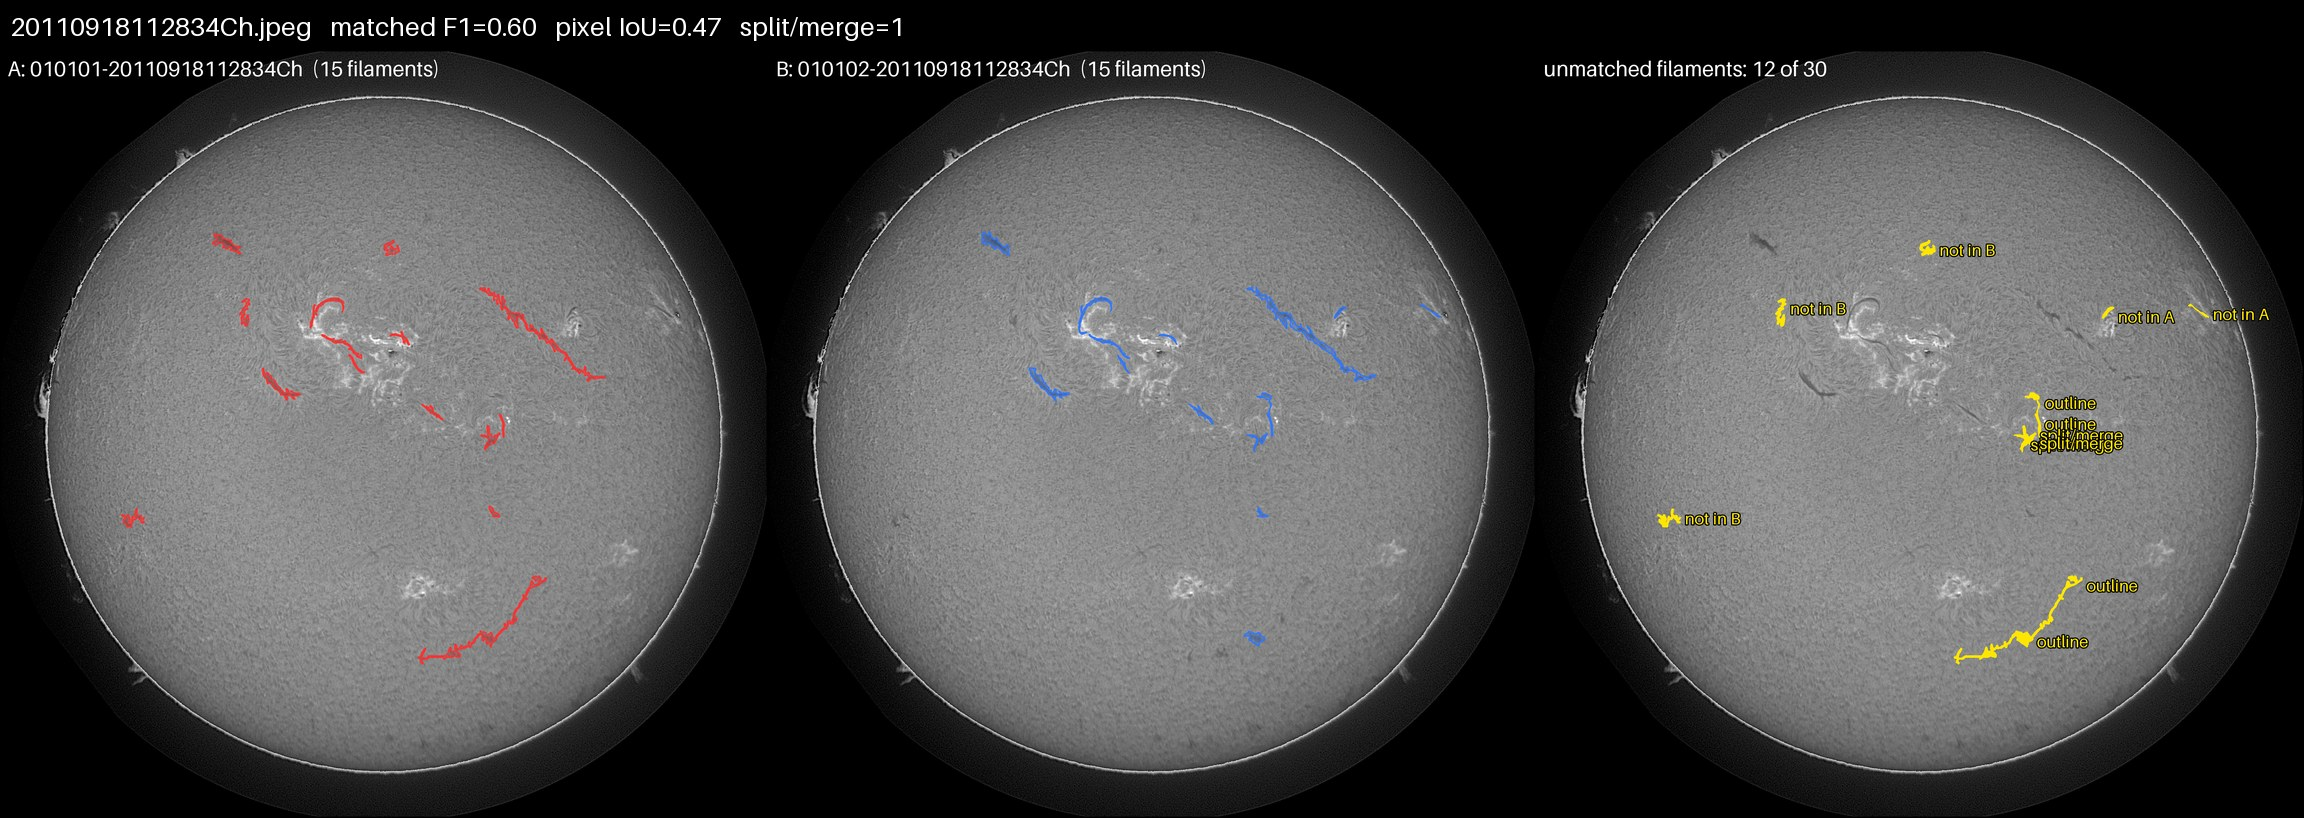
\includegraphics[width=\columnwidth]{figures/disagreement_typical.jpg}
    \caption{Image with median annotator agreement. Left: annotator A; middle: annotator B; right: filaments without a match in the other set, labelled with the reason.}
    \label{fig:agreement}
\end{figure}

\subsection{Results}
    Table~\ref{tab:results} compares the methods. The two-stage pipeline improves validation PQ by 0.045 over the global U-Net and the public score by 0.05; the gain comes from recognition (RQ 0.605\,$\rightarrow$\,0.650) and fewer merged filaments (45\,$\rightarrow$\,33), with SQ also rising (0.666\,$\rightarrow$\,0.690). With ground-truth boxes the segmenter reaches PQ 0.686 (SQ 0.711, RQ 0.965): given the right box it almost always produces a matching mask. Replacing them with detections drops RQ to 0.650 while SQ barely changes, so the remaining gap is detection. The detector saturates near the inter-annotator level: YOLO11s at 1024\,px reaches box precision/recall 0.637/0.647 and YOLO11m at 1536\,px 0.671/0.642, with the same end-to-end PQ (0.447 vs.\ 0.448) at about 4$\times$ the training cost. At the selected setting, 762 of the 1{,}257 validation filaments are matched, with 326 FP, 50 splits and 33 merges.

\begin{table}[t]
    \caption{Validation PQ (113 images, 192 annotation sets, pooled) and public leaderboard score.}
    \label{tab:results}
    \small
    \begin{tabularx}{\columnwidth}{Xccc}
        \toprule
        Method & PQ & SQ / RQ & Public \\
        \midrule
        Global U-Net + components & 0.403 & 0.666 / 0.605 & 0.34 \\
        Two-stage, YOLO11s @ 1024 & 0.447 & -- & 0.39 \\
        Two-stage, YOLO11m @ 1536 & 0.448 & 0.690 / 0.650 & -- \\
        \quad retrained on all images & -- & -- & 0.38 \\
        \midrule
        \emph{Ground-truth boxes} & \emph{0.686} & \emph{0.711 / 0.965} & -- \\
        \bottomrule
    \end{tabularx}
\end{table}

    \textbf{Sensitivity and uncertainty.} The detector confidence threshold matters most: PQ is 0.367, 0.419, 0.436, 0.424 and 0.403 for thresholds 0.1 to 0.5 (mask threshold 0.5, NMS 0.5). Lowering the mask-NMS IoU from 0.7 to 0.3 raises PQ from 0.418 to 0.448 by removing duplicate detections (splits 116\,$\rightarrow$\,50); the mask threshold (0.4--0.6) and minimum area (100--300\,px) change PQ by less than 0.007. Two independent training runs of the segmenter give oracle PQ 0.6975 and 0.6963, which sets the run-to-run spread for the loss comparison in Table~\ref{tab:loss}. The final models predict 17\% more filaments on the test set at the same threshold; raising it to 0.4 restores the earlier count but leaves the public score at 0.38, so we keep the validated setting and attribute the 0.01 gap to leaderboard resolution (two decimals, partial test set).

\begin{table}[t]
    \caption{Loss ablation for the per-filament model (oracle PQ, validation).}
    \label{tab:loss}
    \small
    \begin{tabular}{lc}
        \toprule
        Loss & Oracle PQ \\
        \midrule
        BCE + Dice (two runs) & 0.6975 / 0.6963 \\
        + Lov\'asz hinge \cite{berman2018lovasz} & 0.6981 \\
        + clDice \cite{shit2021cldice} & 0.6839 \\
        \bottomrule
    \end{tabular}
\end{table}

    Lov\'asz hinge, which optimises IoU directly, stays within the run-to-run spread. clDice, designed for tubular structures, lowers oracle PQ by 0.013: it rewards a continuous centreline, whereas annotators draw filaments as loose bands and PQ measures overlap with those bands.

\begin{figure*}[t]
    \centering
    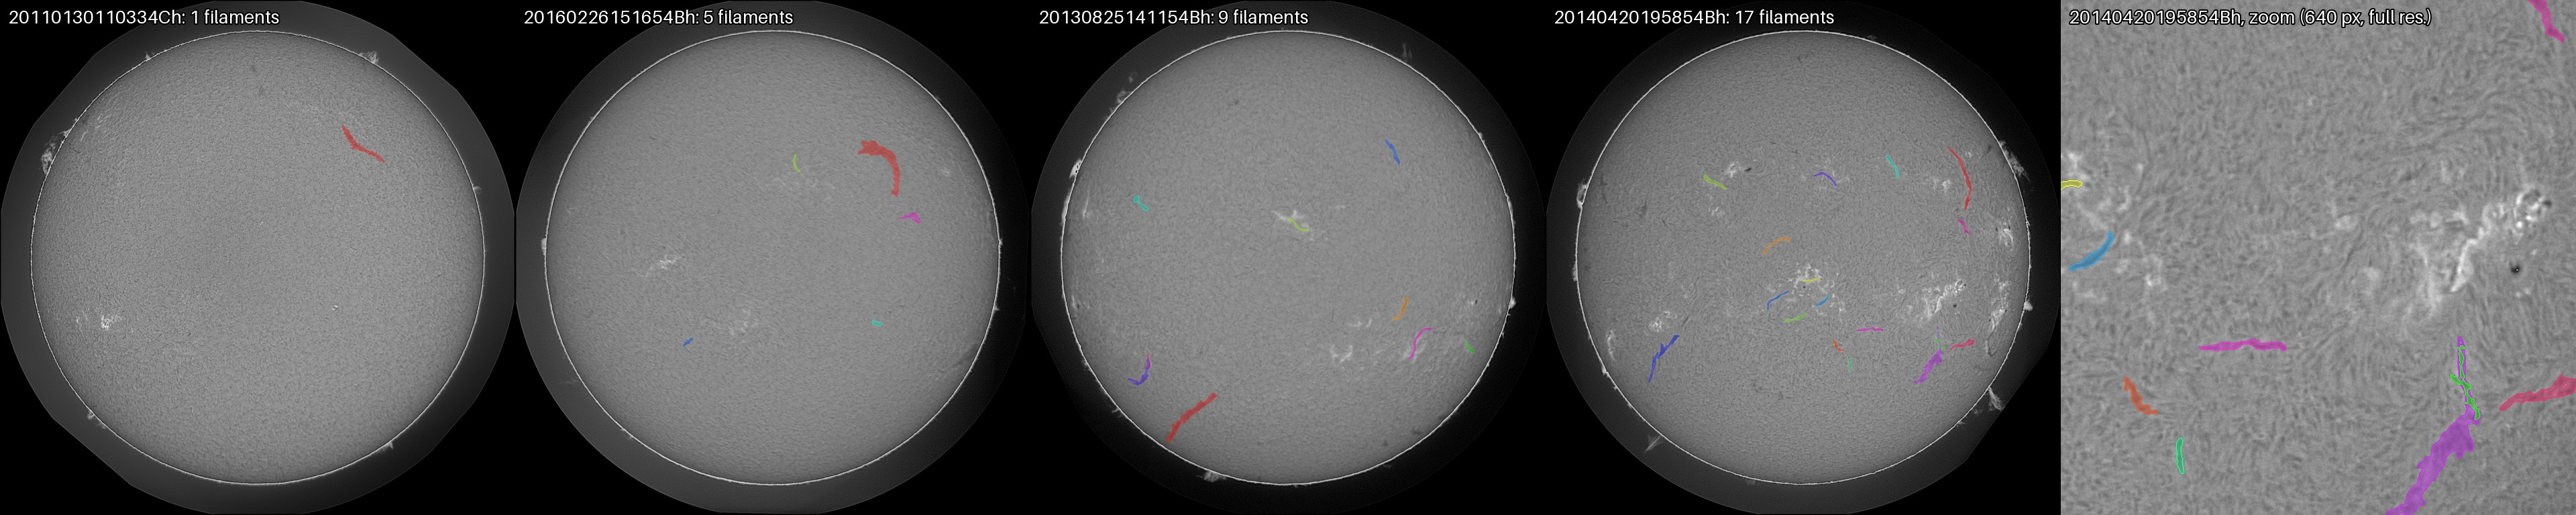
\includegraphics[width=\textwidth]{figures/test_predictions.jpg}
    \caption{Final-model predictions on test images, from fewest to most filaments; one colour per filament. Right: full-resolution zoom of the busiest image.}
    \label{fig:examples}
\end{figure*}

\subsection{Strengths, weaknesses and improvements}
    \textbf{Strengths.} Masks follow the dark material of clearly visible filaments, including long curved filaments near the limb, and neighbouring filaments stay separate (Fig.~\ref{fig:examples}). The segmenter is close to its ceiling given a correct box, training is short (the segmenter trains in 11\,min), and inference is fast (0.31\,s per image).
    \textbf{Weaknesses.} Thin side branches or the faint end of a large filament are sometimes returned as extra small instances next to the main mask, and short dark lanes inside bright active regions are occasionally detected as filaments. Both are among the cases where annotators disagree most, which also limits what any detector can gain against a single annotator's labels.
    \textbf{Improvements.} Oriented boxes would fit long diagonal filaments more tightly; fusing several detectors could add recall; and a learned merging step could join fragments of the same filament that the detector splits.


% ==================================== %
%            ACKNOWLEDGMENT            %
% ==================================== %
\section{Acknowledgment}\label{sec:acknowledgment}
    % Do not change
    The organization of the Filament Segmentation Challenge 2026 is partially supported by the U.S. National Science Foundation (NSF) under Grant No. 2209912 and 2433781, directorate for Computer and Information Science and Engineering (CSE), and Office of Advanced Cyberinfrastructure (OAC), and Grant No. 2511630, AST Division Of Astronomical Sciences and MPS Directorate for Mathematical and Physical Sciences.

    The Filament Segmentation Challenge 2026 is sponsored by the U.S. National Science Foundation (NSF) National Solar Observatory (NSO). 

    This work utilizes GONG data obtained by the NSO Integrated Synoptic Program, managed by the National Solar Observatory, which is operated by the Association of Universities for Research in Astronomy (AURA), Inc. under a cooperative agreement with the National Science Foundation and with contribution from the National Oceanic and Atmospheric Administration. The GONG network of instruments is hosted by the Big Bear Solar Observatory, High Altitude Observatory, Learmonth Solar Observatory, Udaipur Solar Observatory, Instituto de Astrofísica de Canarias, and Cerro Tololo Interamerican Observatory.

\bibliographystyle{ACM-Reference-Format}
\bibliography{main}

\end{document}
